% Options for packages loaded elsewhere
\PassOptionsToPackage{unicode}{hyperref}
\PassOptionsToPackage{hyphens}{url}
\PassOptionsToPackage{dvipsnames,svgnames,x11names}{xcolor}
%
\documentclass[
  number,
  preprint,
  3p]{elsarticle}

\usepackage{amsmath,amssymb}
\usepackage{iftex}
\ifPDFTeX
  \usepackage[T1]{fontenc}
  \usepackage[utf8]{inputenc}
  \usepackage{textcomp} % provide euro and other symbols
\else % if luatex or xetex
  \usepackage{unicode-math}
  \defaultfontfeatures{Scale=MatchLowercase}
  \defaultfontfeatures[\rmfamily]{Ligatures=TeX,Scale=1}
\fi
\usepackage{lmodern}
\ifPDFTeX\else  
    % xetex/luatex font selection
\fi
% Use upquote if available, for straight quotes in verbatim environments
\IfFileExists{upquote.sty}{\usepackage{upquote}}{}
\IfFileExists{microtype.sty}{% use microtype if available
  \usepackage[]{microtype}
  \UseMicrotypeSet[protrusion]{basicmath} % disable protrusion for tt fonts
}{}
\makeatletter
\@ifundefined{KOMAClassName}{% if non-KOMA class
  \IfFileExists{parskip.sty}{%
    \usepackage{parskip}
  }{% else
    \setlength{\parindent}{0pt}
    \setlength{\parskip}{6pt plus 2pt minus 1pt}}
}{% if KOMA class
  \KOMAoptions{parskip=half}}
\makeatother
\usepackage{xcolor}
\setlength{\emergencystretch}{3em} % prevent overfull lines
\setcounter{secnumdepth}{5}
% Make \paragraph and \subparagraph free-standing
\ifx\paragraph\undefined\else
  \let\oldparagraph\paragraph
  \renewcommand{\paragraph}[1]{\oldparagraph{#1}\mbox{}}
\fi
\ifx\subparagraph\undefined\else
  \let\oldsubparagraph\subparagraph
  \renewcommand{\subparagraph}[1]{\oldsubparagraph{#1}\mbox{}}
\fi


\providecommand{\tightlist}{%
  \setlength{\itemsep}{0pt}\setlength{\parskip}{0pt}}\usepackage{longtable,booktabs,array}
\usepackage{calc} % for calculating minipage widths
% Correct order of tables after \paragraph or \subparagraph
\usepackage{etoolbox}
\makeatletter
\patchcmd\longtable{\par}{\if@noskipsec\mbox{}\fi\par}{}{}
\makeatother
% Allow footnotes in longtable head/foot
\IfFileExists{footnotehyper.sty}{\usepackage{footnotehyper}}{\usepackage{footnote}}
\makesavenoteenv{longtable}
\usepackage{graphicx}
\makeatletter
\def\maxwidth{\ifdim\Gin@nat@width>\linewidth\linewidth\else\Gin@nat@width\fi}
\def\maxheight{\ifdim\Gin@nat@height>\textheight\textheight\else\Gin@nat@height\fi}
\makeatother
% Scale images if necessary, so that they will not overflow the page
% margins by default, and it is still possible to overwrite the defaults
% using explicit options in \includegraphics[width, height, ...]{}
\setkeys{Gin}{width=\maxwidth,height=\maxheight,keepaspectratio}
% Set default figure placement to htbp
\makeatletter
\def\fps@figure{htbp}
\makeatother

\usepackage{booktabs}
\usepackage{longtable}
\usepackage{array}
\usepackage{multirow}
\usepackage{wrapfig}
\usepackage{float}
\usepackage{colortbl}
\usepackage{pdflscape}
\usepackage{tabu}
\usepackage{threeparttable}
\usepackage{threeparttablex}
\usepackage[normalem]{ulem}
\usepackage{makecell}
\usepackage{xcolor}
\usepackage{algorithm}
\usepackage{amsmath}
\usepackage{amsthm}
\usepackage{amssymb}
\theoremstyle{plain}
\newtheorem{assumption}{\protect\assumptionname}
\newtheorem{claim}{\protect\claimname}
\newtheorem{condition}{\protect\conditionname}
\newtheorem{conjecture}{\protect\conjecturename}
\newtheorem{cor}{\protect\corollaryname}
\newtheorem{defn}{\protect\definitionname}
\newtheorem{example}{\protect\examplename}
\newtheorem{lem}{\protect\lemmaname}
\newtheorem{notation}{\protect\notationname}
\newtheorem{problem}{\protect\problemname}
\newtheorem{prop}{\protect\propositionname}
\newtheorem{rem}{\protect\remarkname}
\newtheorem{thm}{\protect\theoremname}
\providecommand{\assumptionname}{Assumption}
\providecommand{\claimname}{Claim}
\providecommand{\conditionname}{Condition}
\providecommand{\conjecturename}{Conjecture}
\providecommand{\corollaryname}{Corollary}
\providecommand{\definitionname}{Definition}
\providecommand{\examplename}{Example}
\providecommand{\lemmaname}{Lemma}
\providecommand{\notationname}{Notation}
\providecommand{\problemname}{Problem}
\providecommand{\propositionname}{Proposition}
\providecommand{\remarkname}{Remark}
\providecommand{\theoremname}{Theorem}
\makeatletter
\@ifpackageloaded{tcolorbox}{}{\usepackage[skins,breakable]{tcolorbox}}
\@ifpackageloaded{fontawesome5}{}{\usepackage{fontawesome5}}
\definecolor{quarto-callout-color}{HTML}{909090}
\definecolor{quarto-callout-note-color}{HTML}{0758E5}
\definecolor{quarto-callout-important-color}{HTML}{CC1914}
\definecolor{quarto-callout-warning-color}{HTML}{EB9113}
\definecolor{quarto-callout-tip-color}{HTML}{00A047}
\definecolor{quarto-callout-caution-color}{HTML}{FC5300}
\definecolor{quarto-callout-color-frame}{HTML}{acacac}
\definecolor{quarto-callout-note-color-frame}{HTML}{4582ec}
\definecolor{quarto-callout-important-color-frame}{HTML}{d9534f}
\definecolor{quarto-callout-warning-color-frame}{HTML}{f0ad4e}
\definecolor{quarto-callout-tip-color-frame}{HTML}{02b875}
\definecolor{quarto-callout-caution-color-frame}{HTML}{fd7e14}
\makeatother
\makeatletter
\@ifpackageloaded{caption}{}{\usepackage{caption}}
\AtBeginDocument{%
\ifdefined\contentsname
  \renewcommand*\contentsname{Table of contents}
\else
  \newcommand\contentsname{Table of contents}
\fi
\ifdefined\listfigurename
  \renewcommand*\listfigurename{List of Figures}
\else
  \newcommand\listfigurename{List of Figures}
\fi
\ifdefined\listtablename
  \renewcommand*\listtablename{List of Tables}
\else
  \newcommand\listtablename{List of Tables}
\fi
\ifdefined\figurename
  \renewcommand*\figurename{Figure}
\else
  \newcommand\figurename{Figure}
\fi
\ifdefined\tablename
  \renewcommand*\tablename{Table}
\else
  \newcommand\tablename{Table}
\fi
}
\@ifpackageloaded{float}{}{\usepackage{float}}
\floatstyle{ruled}
\@ifundefined{c@chapter}{\newfloat{codelisting}{h}{lop}}{\newfloat{codelisting}{h}{lop}[chapter]}
\floatname{codelisting}{Listing}
\newcommand*\listoflistings{\listof{codelisting}{List of Listings}}
\makeatother
\makeatletter
\makeatother
\makeatletter
\@ifpackageloaded{caption}{}{\usepackage{caption}}
\@ifpackageloaded{subcaption}{}{\usepackage{subcaption}}
\makeatother
\journal{Journal of Multivariate Analysis}
\ifLuaTeX
  \usepackage{selnolig}  % disable illegal ligatures
\fi
\usepackage[]{natbib}
\bibliographystyle{elsarticle-num-names}
\usepackage{bookmark}

\IfFileExists{xurl.sty}{\usepackage{xurl}}{} % add URL line breaks if available
\urlstyle{same} % disable monospaced font for URLs
\hypersetup{
  pdftitle={Studying the Performance of the Jellyfish Search Optimiser for the Application of Projection Pursuit},
  pdfauthor={H. Sherry Zhang; Dianne Cook; Nicolas Langrené; Jessica Wai Yin Leung},
  pdfkeywords={projection pursuit, jellyfish search optimiser
(JSO), optimisation, grand tour, high-dimensional data, exploratory data
analysis},
  colorlinks=true,
  linkcolor={blue},
  filecolor={Maroon},
  citecolor={Blue},
  urlcolor={Blue},
  pdfcreator={LaTeX via pandoc}}

\setlength{\parindent}{6pt}
\begin{document}

\begin{frontmatter}
\title{Studying the Performance of the Jellyfish Search Optimiser for
the Application of Projection Pursuit}
\author[1]{H. Sherry Zhang%
\corref{cor1}%
}
 \ead{huize.zhang@austin.utexas.edu} 
\author[2]{Dianne Cook%
%
}
 \ead{dicook@monash.edu} 
\author[3]{Nicolas Langrené%
%
}
 \ead{nicolaslangrene@uic.edu.cn} 
\author[2]{Jessica Wai Yin Leung%
%
}
 \ead{Jessica.Leung@monash.edu} 

\affiliation[1]{organization={University of Texas at Austin, Department
of Statistics and Data Sciences},city={Austin},country={United
States},countrysep={,},postcode={78751},postcodesep={}}
\affiliation[2]{organization={Monash University, Department of
Econometrics and Business
Statistics},city={Melbourne},country={Australia},countrysep={,},postcode={3800},postcodesep={}}
\affiliation[3]{organization={Guangdong Provincial Key Laboratory of
Interdisciplinary Research and Application for Data Science,
BNU-HKBU~United~International~College, Department of Mathematical
Sciences},city={Zhuhai},country={China},countrysep={,},postcode={519087},postcodesep={}}

\cortext[cor1]{Corresponding author}




        
\begin{abstract}
The projection pursuit (PP) guided tour interactively optimises a
criteria function known as the PP index, to explore high-dimensional
data by revealing interesting projections. The optimisation in PP can be
non-trivial, involving non-smooth functions and optima with a small
``squint angle'', detectable only from close proximity. To address these
challenges, this study investigates the performance of a recently
introduced swarm-based algorithm, Jellyfish Search Optimiser (JSO), for
optimising PP indexes. The performance of JSO for visualising data is
evaluated across various hyper-parameter settings and compared with
existing optimisers. Additionally, this work proposes novel methods to
quantify two properties of the PP index --~smoothness and
squintability~-- that capture the complexities inherent in PP
optimisation problems. These two metrics are evaluated along with JSO
hyper-parameters to determine their effects on JSO success rate. Our
numerical results confirm the positive impact of these metrics on the
JSO success rate, with squintability being the most significant. The JSO
algorithm has been implemented in the \texttt{tourr} package and
functions to calculate smoothness and squintability are available in the
\texttt{ferrn} package.
\end{abstract}





\begin{keyword}
    projection pursuit \sep jellyfish search optimiser
(JSO) \sep optimisation \sep grand tour \sep high-dimensional data \sep 
    exploratory data analysis
\end{keyword}
\end{frontmatter}
    
\section{Introduction}\label{introduction}

Projection Pursuit (PP) (\citet{kr69}, \citet{FT74}) is a dimension
reduction technique aimed at identifying informative linear projections
of data. The method involves optimising an objective function known as
the PP index (e.g. \citet{hall1989polynomial},
\citet{cook1993projection}, \citet{lee2010projection},
\citet{Loperfido2018}, \citet{Loperfido2020}), which defines the
criteria for what constitutes interesting or informative projections.
Let \(X \in \mathbb{R}^{n\times p}\) be the data matrix,
\(A \in\mathbb{R}^{p \times d}\) be an orthonormal matrix, where \(A\)
belongs to the Stiefel manifold \(\mathcal{A} = V_d(\mathbb{R}^p)\). The
projection \(Y = XA\) is a linear transformation that maps data from a
\(p\)-dimensional space into a \(d\)-dimensional space. The index
function \(f(XA): \mathbb{R}^{n \times d} \to \mathbb{R}\) is a scalar
function that measures an interesting aspect of the projected data, such
as deviation from normality, presence of clusters, non-linear structure,
or other features of interest. For a fixed data, PP finds the
orthonormal basis \(A\) that maximises the index value of the
projection, \(Y = XA\):

\begin{equation}\phantomsection\label{eq-optimization}{
\underset{A \in \mathcal{A}}{\max } \quad f(XA) \quad \text{subject to} \quad A'A = I_d
}\end{equation}

The index functions can be non-linear and non-convex, hence an effective
and efficient optimisation procedure is essential to explore the data
landscape and achieve a globally optimal viewpoint of the data.

Optimisation of PP is typically investigated in the literature when new
indexes are proposed \citep{posse1995, marie-sainte2010, grochowski2011}
or when visualisation method are used to track the optimisation process.
\citet{cook1995grand} introduced the PP guided tour, which monitors the
optimisation visually to see the data projections leading in and out of
the optima. An implementation is available in the \texttt{tourr} package
\citep{tourr} in R \citep{R}. \citet{RJ-2021-105} illustrated how to
diagnose optimisation processes, particularly focusing on the guided
tour, and revealed a need for improved optimisation. While improving the
quality of the optimisation solutions in the tour is essential, it is
also important to be able to view the data projections as the
optimisation progresses. Integrating the guided tour with a global
optimisation algorithm that is efficient in finding the global optimal
and enables viewing of the projected data during the exploration process
is a goal.

Here, the potential for a Jellyfish Search Optimiser (JSO) to be
integrated with the projection pursuit guided tour is explored. JSO,
\citep{chou_novel_2021} - \citep{rajwar_exhaustive_2023}, inspired by
the search behaviour of jellyfish in the ocean, is a swarm-based
metaheuristic designed to solve global optimisation problems. Compared
to traditional methods, JSO has demonstrated stronger search ability and
faster convergence, and requires fewer tuning parameters. These
practical advantages make JSO a promising candidate for enhancing PP
optimisation.

The primary goal of the study reported here is to investigate the
performance of JSO in PP optimisation for the guided tour. It is of
interest to assess how quickly and closely the optimiser reaches a gobal
optima, for various PP indexes that may have differing complexities. To
observe the performance of JSO with different types of PP indexes,
metrics are introduced to capture specific properties of the index
including squintability (based on \citet{barnett1981interpreting}'s
squint angle) and smoothness as introduced in \citet{laa_using_2020}.
Here we mathematically define metrics for squintability and smoothness,
which is new for the field. A series of simulation experiments using
various datasets and PP indexes are conducted to assess JSO's behaviour
and its sensitivity to hyper-parameter choices (number of jellyfish and
maximum number of tries). The relationship between the JSO performance,
hyper-parameter choices and properties of PP indexes (smoothness and
squintability) is analysed to provide guidance on selecting optimisers
for practitioners using projection pursuit. Additionally, it aims to
guide the design of new indexes that facilitate easy optimization for PP
researchers.

The paper is structured as follows. Section~\ref{sec-background}
introduces the background of PP guided tour and reviews existing
optimisers and index functions in the literature.
Section~\ref{sec-theory} details JSO and introduces metrics that measure
different properties of PP indexes, smoothness and squintability.
Section~\ref{sec-sim-deets} details two simulation experiments to assess
JSO's performance: one comparing JSO's performance improvements relative
to an existing optimiser, Creeping Random Search (CRS), and the other
studying the impact of different PP index properties on optimisation
performance. Section~\ref{sec-sim-res} presents the results.
Section~\ref{sec-conclusion} summarises the work and provides
suggestions for future directions.

\section{Projection pursuit, tours, index functions and
optimisation}\label{sec-background}

A tour on high-dimensional data is constructed by geodesically
interpolating between pairs of planes. Any plane is described by an
orthonormal basis, \(A_t\), where \(t\) represents time in the sequence.
The term ``geodesic'' refers to maintaining the orthonormality
constraint so that each view shown is correctly a projection of the
data. The PP guided tour operates by geodesically interpolating to
target planes (projections) which have high PP index values, as provided
by the optimiser. The geodesic interpolation means that the viewer sees
a continuous sequence of projections of the data, so they can watch
patterns of interest forming as the function is optimised. There are
five (unsophisticated) optimisation methods implemented in the
\texttt{tourr} package:

\begin{itemize}
\tightlist
\item
  \texttt{search\_geodesic()}: provides a pseudo-derivative
  optimisation. It searches locally for the best direction, based on
  differencing the index values for very close projections. Then it
  follows the direction along the geodesic path between planes, stopping
  when the next index value fails to increase.
\item
  \texttt{search\_better()}: also known as Creeping Random Search (CRS),
  is a brute-force optimisation searching randomly for projections with
  higher index values.
\item
  \texttt{search\_better\_random()}: is essentially simulated annealing
  \citep{Bertsimas93} where the search space is reduced as the
  optimisation progresses.
\item
  \texttt{search\_posse()}: implements the algorithm described in
  \citet{posse95}.
\item
  \texttt{search\_polish()}: is a very localised search, to take tiny
  steps to get closer to the local maximum.
\end{itemize}

There are several PP index functions available: \texttt{holes()} and
\texttt{cmass()} \citep{cook1993projection}; \texttt{lda\_pp()}
\citep{lee2005projection}; \texttt{pda\_pp()} \citep{lee2010projection};
\texttt{dcor2d()} and \texttt{splines2d()} \citep{Grimm2016};
\texttt{norm\_bin()} and \texttt{norm\_kol()} \citep{huber85};
\texttt{slice\_index()} \citep{Laa:2020wkm}. Most are relatively simply
defined, for any projection dimension, and implemented because they are
relatively easy to optimise. A goal is to be able to incorporate more
complex PP indexes, for example, based on scagnostics (\citet{scag},
\citet{WW08}).

An initial investigation of PP indexes, and the potential for
scagnostics is described in \citet{laa_using_2020}. To be useful here an
optimiser needs to be able to handle index functions which are possibly
not very smooth. In addition, because data structures might be
relatively fine, the optimiser needs to be able to find maxima that
occur with a small squint angle, that can only be seen from very close
by. One last aspect that is useful is for an optimiser to return local
maxima in addition to global because data can contain many different and
interesting features.

\section{The jellyfish optimiser and properties of PP
indexes}\label{sec-theory}

JSO mimics the natural movements of jellyfish, which include passive and
active motions driven by ocean currents and their swimming patterns,
respectively. In the context of optimization, these movements are
abstracted to explore the search space, aiming to balance exploration
(searching new areas) and exploitation (focusing on promising areas).
The algorithm aims to find the optimal solution by adapting the
behaviour of jellyfish to navigate towards the best solution over
iterations \citep{chou_novel_2021}.

To solve the optimisation problem embedded in the PP guided tour, a
starting projection, an index function, the number of jellyfish, and the
maximum number of trials (tries) are provided as input. Then, the
current projection is evaluated by the index function. The projection is
then moved in a direction determined by a random factor, influenced by
how far along we are in the optimisation process. Occasionally,
completely new directions may be taken like a jellyfish might with ocean
currents. A new projection is accepted if it is an improvement compared
to the current one, rejected otherwise. This process continues and
iteratively improves the projection, until the pre-specified maximum
number of trials is reached.

\begin{tcolorbox}[enhanced jigsaw, leftrule=.75mm, colbacktitle=quarto-callout-note-color!10!white, titlerule=0mm, toprule=.15mm, bottomtitle=1mm, toptitle=1mm, arc=.35mm, coltitle=black, left=2mm, breakable, title={Algorithm: Jellyfish Optimizer Pseudo Code}, colframe=quarto-callout-note-color-frame, rightrule=.15mm, bottomrule=.15mm, opacitybacktitle=0.6, colback=white, opacityback=0]

\textbf{Input}: \texttt{current\_projections}, \texttt{index\_function},
\texttt{trial\_id}, \texttt{max\_trial}

\textbf{Output}: \texttt{optimised\_projection}

\textbf{Initialize} \texttt{current\_best} as the projection with the
best index value from \texttt{current\_projections}, and
\texttt{current\_idx} as the array of index values for each projection
in \texttt{current\_projections}

\textbf{for} each \texttt{trial\_id} in 1 to \texttt{max\_tries}
\textbf{do}

\begin{quote}
Calculate the time control value, \(c_t\), based on
\texttt{current\_idx} and \texttt{max\_trial}
\end{quote}

\begin{quote}
\textbf{if} \(c_t\) is greater than or equal to \(0.5\) \textbf{then}

\begin{quote}
Define trend based on the \texttt{current\_best} and
\texttt{current\_projections}
\end{quote}

\begin{quote}
Update each projection towards the trend using a random factor and
orthonormalisation
\end{quote}

\textbf{else}

\begin{quote}
\textbf{if} a random number is greater than \(1 - c_t\) \textbf{then}

\begin{quote}
Slightly adjust each projection with a small random factor (passive)
\end{quote}

\textbf{else}

\begin{quote}
For each projection, compare with a random jellyfish and adjust towards
or away from it (active)
\end{quote}
\end{quote}

Update the orientation of each projection to maintain consistency

Evaluate the new projections using the index function
\end{quote}

\begin{quote}
\textbf{if} any new projection is worse than the current, revert to the
\texttt{current\_projections} for that case

\begin{quote}
Determine the projection with the best index value as the new
\texttt{current\_best}
\end{quote}
\end{quote}

\begin{quote}
\textbf{if} \texttt{trial\_id} \(\ge\) \texttt{max\_trial}, print the
last best projection \textbf{exit}
\end{quote}

\textbf{return} the set of projections with the updated
\texttt{current\_best} as the \texttt{optimised\_projection}

\end{tcolorbox}

The JSO implementation involves several key parameters that control its
search process in optimization problems. These parameters are designed
to guide the exploration and exploitation phases of the algorithm. While
the specific implementation details can vary depending on the version of
the algorithm or its application, the focus is on two main parameters
that are most relevant to our application: the number of jellyfish and
the maximum number of tries.

\citet{laa_using_2020} has proposed five criteria for assessing
projection pursuit indexes (smoothness, squintability, flexibility,
rotation invariance, and speed). Since not all index properties affect
the optimisation process, the focus here is on the first two properties,
\emph{smoothness} (Section~\ref{sec-smoothness}) and
\emph{squintability} (Section~\ref{sec-squintability}), for which
metrics are proposed to quantify them.

\subsection{Smoothness}\label{sec-smoothness}

This subsection proposes a metric for the smoothness of a projection
pursuit index.

An classical way to describe the smoothness of a function is to identify
how many continuous derivatives of the function exist. This can be
characterized by Sobolev spaces \citep{adams2003sobolev}.

\begin{defn}\label{def:sobolev_space}
The Sobolev space $W^{k,p}(\mathbb{R})$ for $1\leq p\leq \infty$ is the set of all functions $f$ in $L^p(\mathbb{R})$ for which all weak derivatives $f^{(\ell)}$ of order $\ell\leq k$ exist and have a finite $L^p$ norm.
\end{defn}

The Sobolev index \(k\) in Definition \ref{def:sobolev_space} can be
used to characterize the smoothness of a function: if \(f\in W^{k,p}\),
then the higher \(k\), the smoother \(f\). While this Sobolev index
\(k\) is a useful measure of smoothness, it can be difficult to compute
or even estimate in practice.

To obtain a computable estimator of the smoothness of the index function
\(f\), we propose an approach based on random fields. If a PP index
function \(f\) is evaluated at some random bases, as is done at the
initialization stage of JSO, then these random index values can be
interpreted as a random field, indexed by a space parameter, namely the
random projection basis. This analogy suggests to use this random
training sample to fit a spatial model. We propose to use a Gaussian
process equipped with a Matérn covariance function, due to the
connections between this model and Sobolev spaces, see for example
\citet{porcu2024matern}.

The distribution of a Gaussian process is fully determined by its mean
and covariance function. The smoothness property comes into play in the
definition of the covariance function: if a PP index is very smooth,
then two close projection bases should produce close index values
(strong correlation); by contrast, if a PP index is not very smooth,
then two close projection bases might give very different index values
(fast decay of correlations with respect to distance between bases).
Popular covariance functions are parametric positive semi-definite
functions. In particular, the Matérn class of covariance functions has a
dedicated parameter to capture the smoothness of the Gaussian field.

\begin{defn}
The Matérn covariance function $K$ is defined by
\begin{equation}
K(u)=K_{\nu,\eta,\ell}(u):=\eta^2\frac{\left(\sqrt{2\nu}\frac{u}{\ell}\right)^{\nu}}{\Gamma(\nu)2^{\nu-1}}\mathcal{K}_{\nu}\left(\sqrt{2\nu}\frac{u}{\ell}\right)\ , u\geq0\label{eq:matern}
\end{equation}
where $\nu>0$ is the smoothness parameter, $\eta$ is the outputscale, $\ell$ is the lengthscale, and $\mathcal{K}_\nu$ is
the modified Bessel function \citep[10.25]{DLMF}. A multivariate extension $K(u)$, $u\in\mathbb{R}^d$ can be obtained by products of univariate covariance functions \eqref{eq:matern}.
\end{defn}

The Matérn covariance function can be expressed analytically when
\(\nu\) is a half-integer, the most popular values in the literature
being \(\frac{1}{2}\), \(\frac{3}{2}\) and \(\frac{5}{2}\)
\citep{rasmussen2006gaussian}. The parameter \(\nu\), called
\emph{smoothness parameter}, controls the decay of the covariance
function. As such, it is an appropriate measure of smoothness of a
random field. For example, \citet{karvonen2023asymptotic} showed that if
a function \(f\) has a Sobolev index of \(k\), then the smoothness
parameter estimate \(\nu\) in \eqref{eq:matern} cannot be asymptotically
less than \(k\). See the survey \citet{porcu2024matern} for additional
results on the connection between the Matérn model and Sobolev spaces.
An interesting result is that the asymptotic case
\(\nu\rightarrow\infty\) coincides with the Gaussian kernel:
\(K_\infty(u)=\exp(-u^{2}/2)\).

In view of these results, the parameter \(\nu\) is suggested as a
measure of the smoothness of the PP index function by fitting a Gaussian
process prior with Matérn covariance on a dataset generated by random
evaluations of the index function, as done at the initialization stage
of the jellyfish search optimization. There exist several R packages,
such as \texttt{GpGp} \citep{guinness2021gpgp} or \texttt{ExaGeoStatR}
\citep{abdulah2023large}, to fit the hyperparameters of a GP covariance
function on data, which is usually done by maximum likelihood
estimation. In this project, the \texttt{GpGp} package is used.

\begin{defn}
Let $\mathbf{A}=[A_1, \ldots, A_N] \in (\mathbf{R}^{p \times d})^N$ be d-dimensional projection bases, let $\mathbf{y}=[f(XA_1),\ldots,f(XA_N)]$ be the corresponding PP index values, and let $\mathbf{K}=[K_\theta(A_{i},A_{j})]_{1\leq i,j\leq N}\in\mathbb{R}^{N\times N}$ be the Matérn covariance matrix evaluated at the input bases, where the vector $\theta$ contains all the parameters of the multivariate Matérn covariance function $K$ (smoothness, outputscale, lengthscales). The log-likelihood of the parameters $\theta$ is defined by 
\begin{equation}
\mathcal{L}(\theta)=\log p(\mathbf{y}\left|\mathbf{A},\theta\right.)=-\frac{1}{2}\mathbf{y}^{\top}(\mathbf{K}+\sigma^{2}\mathbf{I})^{-1}\mathbf{y}-\frac{1}{2}\mathrm{\log}(\det(\mathbf{K}+\sigma^{2}\mathbf{I}))-\frac{N}{2}\log(2\pi)\,.\label{eq:gp_log_likelihood}
\end{equation}
where the nugget parameter $\sigma$ is the standard deviation of the intrinsic noise of the Gaussian process.
The optimal parameters (including smoothness) are obtained by maximum log-likelihood
\begin{equation}
\theta^* = \underset{\theta}{\max}\mathcal{L}(\theta)
\end{equation}
The resulting optimal smoothness parameter $\nu$ is chosen as our smoothness metric.
\end{defn}

The value of the optimal smoothness parameter \(\nu>0\) can be naturally
interpreted as follows: the higher \(\nu\), the smoother the index
function.

\subsection{Squintability}\label{sec-squintability}

Squintability has been a useful concept. Here, it is defined
mathematically and two approaches to compute this metric numerically,
are described.

\begin{defn}[projection distance]\label{def:proj-dist}
Let $A \in \mathbf{R}^{p \times d}$ be the d-dimensional projection basis and
$A^*$ be the optimal basis that achieves the maximum index value for a given
PP problem defined by the shape to find, data dimension,
and the index function. The projection distance $d(A, A^*)$ between $A$ 
and $A^*$ is defined as 
$d(A, A^*) = \lVert AA^\prime - A^*A^{*\prime}\  \rVert _F$
where $\lVert . \rVert _F$ denotes the Frobenius norm, given by
$\lVert M \rVert _F = \sqrt{\sum_{ij} M_{ij}^2}$. 
\end{defn}

We now focus our attention to how the index value \(f(XA)\) changes with
respect to the projection distance \(d(A, A^*)\), over the course of the
JSO.

\begin{defn}[squintability]\label{def:squintability}
Let $g: \mathbb{R} \mapsto  \mathbb{R}$ be a decreasing function that maps the projection distance, $d = d(A, A^*)$, 
to the index value $f(XA)$, such that $g(d(A, A^*)) = f(XA)$. The squintability of the index function $f(\cdot)$, is defined as 
$$\varsigma(f) = -c \times \max_{d} g'(d) \times \arg \max_{d} g'(d)$$ 
where $c$ is a constant scaling factor, $-\max_d g'(d)$ represents the 
largest gradient of $-g$ and $\arg \max_{d} g'(d)$ represents the projection distance at which this largest gradient is attained.

\end{defn}

\begin{prop}\label{prop:my_prop}
This is a proposition.
\end{prop}

Proposition \ref{prop:my_prop} is useful.

From \citet{barnett1981interpreting} and \citet{laa_using_2020}, a large
squint angle implies that the objective function value is close to
optimal even when the perfect view to see the structure is far away. A
small squint angle means that the PP index value improves substantially
only when the perfect view is close by. As such, low squintability
implies rapid improvement in the index value when near the perfect view.
For PP, a small squint angle is considered to be undesirable because it
means that the optimiser needs to be very close to be able to ``see''
the optima. Thus, it could be difficult for the optimiser to find the
optima. The mathematical formulation of this intuition is proposed
below:

It is expected that for a PP index with high squint angle, the
optimization (\ref{eq-optimization}) should make substantial progress
early on. Conversely, for a PP index with low squint angle, it might
take a long while for the optimization to make substantial progress, as
the candidate projections would need to be very close to the optimal one
for the structure of the index function to be visible enough to be
amenable to efficient optimization. This observation suggests that the
extreme values of \(f'\) (the ones for which \(f''=0\), assuming that
\(f\) is twice differentiable), and the projection distances for which
these values are attained, are crucial in the mathematical definition of
squintability. Noticing that \(f\) is expected to be a decreasing
function, the squintability metric is proposed as follows:

\begin{equation}\phantomsection\label{eq-squintability}{
\varsigma:=-4\min_{x}f'(x)\times\underset{x}{\arg\min}f'(x)\ .
}\end{equation}

\(-\min_{x}f'(x)\) represents the largest value of the gradient of
\(-f\) and \(\underset{x}{\arg\min}f'(x)\) represents the projection
distance at which this largest gradient is attained. It is expected that
these two values should be both high in the case of high squintability
(fast increase in \(f\) early on), and both low in the case of low
squintability (any substantial increase in \(f\) happens very late,
close to the optimal angle). This suggest that their product
(\ref{eq-squintability}) should provide a sensible measure of
squintability. The multiplicative constant \(4\), which can be deemed
arbitrary, does not change the interpretation of the squintability
metric \(\varsigma\); it is here to adjust the range of values of
\(\varsigma\) and simplify the explicit formula for \(\varsigma\)
obtained later on.

To compute the squintability metric (\ref{eq-squintability}) in
practice, several approaches are possible. The first one is to propose a
parametric model for \(f\), and use it to obtain an explicit formula for
\(\varsigma\). Numerical experiments suggest a scaled sigmoid shape as
described below. Define

\begin{equation}\phantomsection\label{eq-logistic}{
\ell(x):=\frac{1}{1+\exp(\theta_{3}(x-\theta_{2}))}\ ,
}\end{equation}

which is a decreasing logistic function depending on two parameters
\(\theta_2\) and \(\theta_3\), such that
\(\ell(\theta_{2})=\frac{1}{2}\). Then, define

\begin{equation}\phantomsection\label{eq-parametric}{
f(x)=(\theta_{1}-\theta_{4})\frac{\ell(x)-\ell(x_{\max})}{\ell(0)-\ell(x_{\max})}+\theta_{4}\ ,
}\end{equation}

which depends on three additional parameters, \(\theta_1\),
\(\theta_2\), and \(x_{\max}\), such that \(f(0)=\theta_1\) and
\(f(x_{\max})=\theta_4\). Under the parametric model
(\ref{eq-parametric}), the squintability metric (\ref{eq-squintability})
can be shown to be equal to

\begin{equation}\phantomsection\label{eq-squintability-parametric}{
\varsigma=\frac{(\theta_{1}-\theta_{4})\theta_{2}\theta_{3}}{\ell(0)-\ell(x_{\max})}\ .
}\end{equation}

In practice, the parameters of this model (\ref{eq-parametric}) can be
estimated numerically, for example by non-linear least squares, and then
used to evaluate \(\varsigma\) as in equation
(\ref{eq-squintability-parametric}).

Alternatively, one can estimate (\ref{eq-squintability}) in a
nonparametric way, for example by fitting \(f\) using kernel regression,
then numerically estimate the angle at which \(-f'\) attains its highest
value.

\section{Simulation details}\label{sec-sim-deets}

The JSO performance is compared with an existing optimiser, Creeping
Random Search (CRS) \citep{RJ-2021-105, laa_using_2020} used in the PP
guided tour to explore JSO's behaviour under different hyper-parameter
and data dimension combinations. The second simulation studies the
effect of index properties (smoothness and squintability), along with
JSO hyper-parameters, and data dimension, on the success rate of the JSO
performance. This section describes the simulation details, with the
results deferred to Section Section~\ref{sec-sim-res}.

\subsection{Performance of JSO relative to CRS}\label{sec-app-1}

he performance of JSO is investigated both in comparison to the existing
optimizer, CRS, and across various hyper-parameter values. The
performance is measured by the success rate, defined as the proportion
of simulations that achieves a final index value within 0.05 of the best
index value found among all 50 simulations (see
Figure~\ref{fig-success-rate} for an illustration). This comparison is
based on projection pursuit to find the pipe shape investigated by
\citet{laa_using_2020} using the \texttt{holes} index.

Fifty simulations are conducted with both JSO and CRS, in four different
data dimensions (\(d = 6, 8, 10, 12\)). JSO uses 100 jellyfishes with a
maximum of 100 tries, while the CRS allows a maximum of 1000 samples at
each iteration before the algorithm terminates. The different numbers
account for the multiple paths of JSO to enable fairer comparison with
CRS. The results of the simulation are collected using the data
structure proposed in \citet{RJ-2021-105} for assessing JSO, where the
design parameters are stored along with index value, projection basis,
random seed, and computation time.

Fifty additional simulations are conducted for each hyper-parameter
combination to analyze how they affect the JSO success rate. This
includes variations in the number of jellyfish (20, 50, and 100) and the
maximum number of tries (50 and 100).

\begin{figure}

\centering{

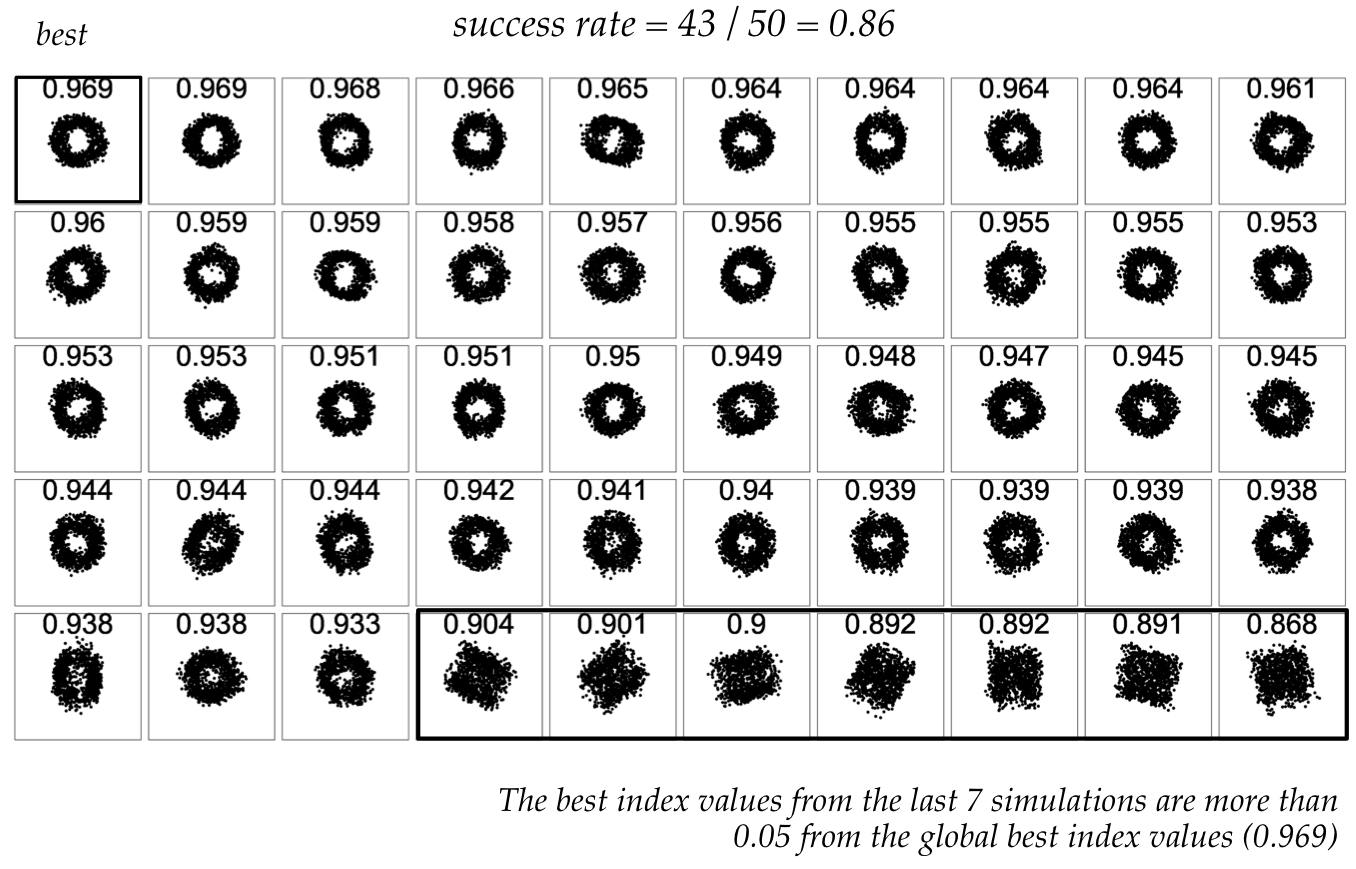
\includegraphics[width=4.52in,height=\textheight]{figures/success-rate.png}

}

\caption{\label{fig-success-rate}Illustration of success rate
calculation: Final projections based on projection pursuit to find the
pipe shape in 8D data using the holes index, optimised by CRS, in 50
simulations. The 50 final projections are sorted by their index values.
The highest index value found across all simulations is 0.969. Out of
the 50 simulations, 43 achieved an index value within 0.05 of the best,
resulting in a success rate of 0.86 (43/50).}

\end{figure}%

\subsection{Factors affecting JSO success rate: index properties and
jellyfish hyper-parameters}\label{sec-app-2}

To assess JSO's performance across various scenarios, two different data
shapes, pipe and a sine wave, are investigated in 6D and 8D spaces using
six different PP indexes: \texttt{dcor2d\_2}, \texttt{loess2d},
\texttt{MIC}, \texttt{TIC}, \texttt{spline}, and \texttt{stringy}, with
varied JSO hyper-parameters. A total of 52 combinations result,
comprising of 24 computed on the pipe data and 28 on the sine-wave data.
Again, JSO is run 50 times to calculate the success rate for each
projection pursuit.

Smoothness and squintability are computed following the procedures
outlined in Section~\ref{sec-smoothness} and
Section~\ref{sec-squintability} and as illustrated in
Figure~\ref{fig-smoothness} and Figure~\ref{fig-squintability}.

To compute smoothness, 300 random bases are simulated. Index values and
projection distance (to the optimal basis) are calculated for each
random basis before fitting the Gaussian process model to obtain the
smoothness measure for the index.

To compute squintability, 50 random bases are sampled and interpolated
to the optimal basis with a step size of 0.005. Index values and
projection distances are calculated for these interpolated bases and the
index values are averaged with a bin width of 0.005. A four-parameter
scaled logistic function is fitted to the index values against
projection distances, estimated by non-linear least squares. The
squintability measure is then calculated as
\ref{eq-squintability-parametric}.

To construct a relationship among success rate, index properties
(smoothness and squintability), and jellyfish hyper-parameters, a
generalised linear model is fitted using a binomial family and a logit
link function. The data is pre-processed by 1) scaling the JSO
hyper-parameters by a factor of 10 for interpretation, 2) creating a new
binary variable \texttt{long\_time} to indicate cases with an average
run time over 30 seconds, and 3) re-coding the success rate for the
\texttt{stringy} index as 0, because none of the 50 simulations
correctly identified the sine-wave shape.

\begin{figure}

\centering{

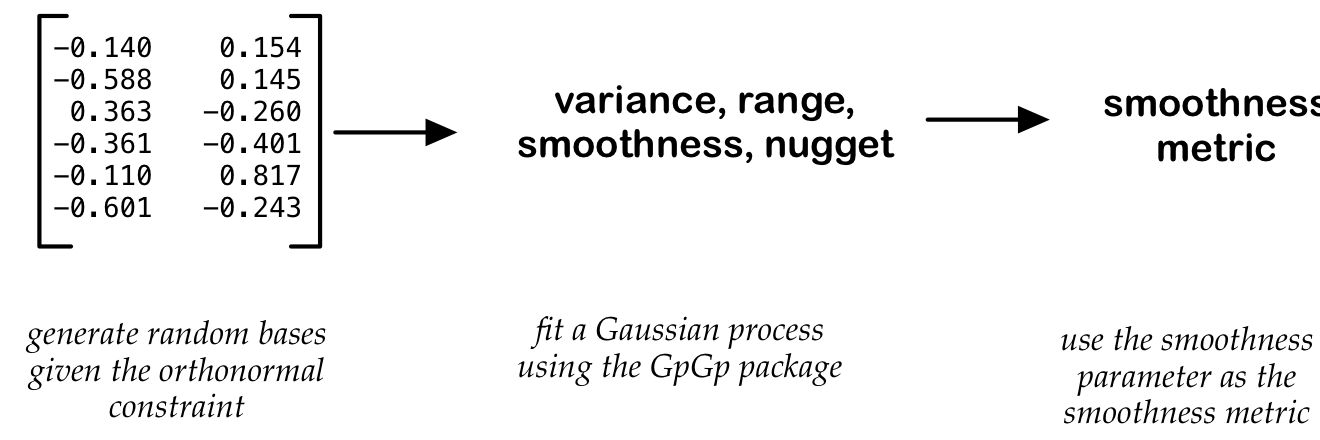
\includegraphics[width=1\textwidth,height=\textheight]{figures/smoothness.png}

}

\caption{\label{fig-smoothness}Illustration of steps to calculate
smoothness. For a given projection pursuit problem defined by the shape
to find, data dimension and the index function, 1) sample random bases
given the orthonormality contraint, 2) calculate the projection distance
and the index value for each random basis, and 3) fit a Gaussian process
model of index values against projection distances to obtain the
smoothness measure.}

\end{figure}%

\begin{figure}

\centering{

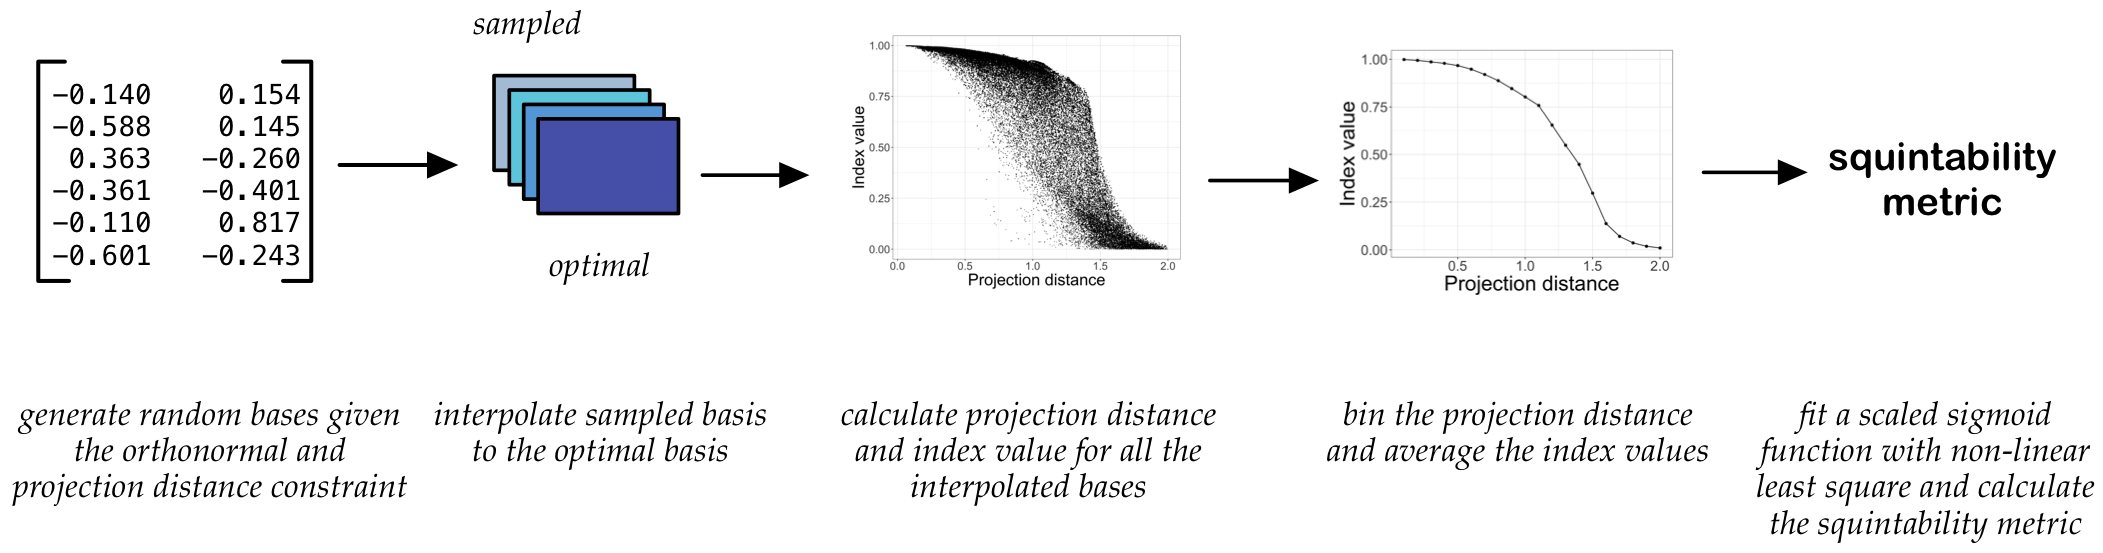
\includegraphics[width=1\textwidth,height=\textheight]{figures/squintability.png}

}

\caption{\label{fig-squintability}Illustration of steps to calculate
squintability. For a given projection pursuit problem defined by the
shape to find, data dimension and the index function, 1) sample random
bases given the orthonormality and projection distance contraint, 2)
interpolate the sampled bases to the optimal basis and calculate the
projection distance and the index value for each interpolated basis. 3)
bin the index values by projection distances to obtain the average index
value for each bin, 4) fit the scaled sigmoid function in Equation
\ref{eq-squintability} to the binned index values against projection
distances using non-linear least square, 5) calculate the squintability
measure using Equation \ref{eq-squintability-parametric} with parameters
estimated from the model.}

\end{figure}%

\section{Results}\label{sec-sim-res}

The results from the first simulation described in
Section~\ref{sec-sim-deets} are analysed based on the final projections
across two optimisers (JSO and CRS) and the success rate across JSO
hyper-parameters. In the second simulation, smoothness and squintability
are calculated across a collection of pipe-finding and sine-wave finding
problems to construct the relationship between success rate, JSO
hyper-parameters, and index properties.

The final projections found by the two optimisers (JSO and CRS) are
presented in Figure~\ref{fig-proj}, broken down by 10th quantile,
faceted by the data dimensions. In the 6-dimensional data scenario, JSO
consistently identifies a clear pipe shape. The CRS also finds the pipe
shape but with a wide rim, suggesting a further polish search may be
required. With increasing dimensions, JSO may not always identify the
pipe shape due to random sampling, but it still finds the pipe shape in
over 50\% of cases. Compared to CRS, JSO achieves higher index values
and clearer pipe shapes across all quantiles in data of 8, 10, 12
dimensions, suggesting its advantage in exploring high-dimensional
spaces.

The success rate calculated at each hyper-parameter combination (number
of jellyfish and the maximum number of tries) is presented in
Figure~\ref{fig-proportion}. As the number of jellyfish and maximum
tries increase, the success rate also increases. For simpler problems (6
dimensions), small parameter values (20 jellyfishes and a maximum of 50
tries) can already achieve a high success rate. However, larger
parameter values (i.e.~100 jellyfishes and a maximum of 100 tries) are
necessary for higher-dimensional problems (8, 10, and 12 dimensions).
Increasing both parameters enhances the performance of JSO, but it also
extends the computational time required for the optimisation, which can
be computationally intensive when evaluating the index function (such as
scagnostic indexes) multiple times across numerous iterations.

\begin{figure}

\centering{

\includegraphics{jso_files/figure-pdf/fig-proj-1.pdf}

}

\caption{\label{fig-proj}Projections found by the JSO and CRS at each
10th quantile across 50 simulations. The projection pursuit problem is
to find the pipe shape using the holes index in the 6, 8, 10, and
12-dimensional spaces. The JSO uses 100 jellyfishes and a maximum number
of tries of 100. The CRS uses a maximum of 1000 tries in each step of
random sampling step before the algorithm terminates. In the 6-D data
space, JSO always finds a clear pipe shape while the CRS also finds the
pipe shape but with a wide rim. At higher data dimensions, JSO finds a
higher index value and a clearer pipe shape across all the quantiles
than the CRS}

\end{figure}%

\begin{figure}

\centering{

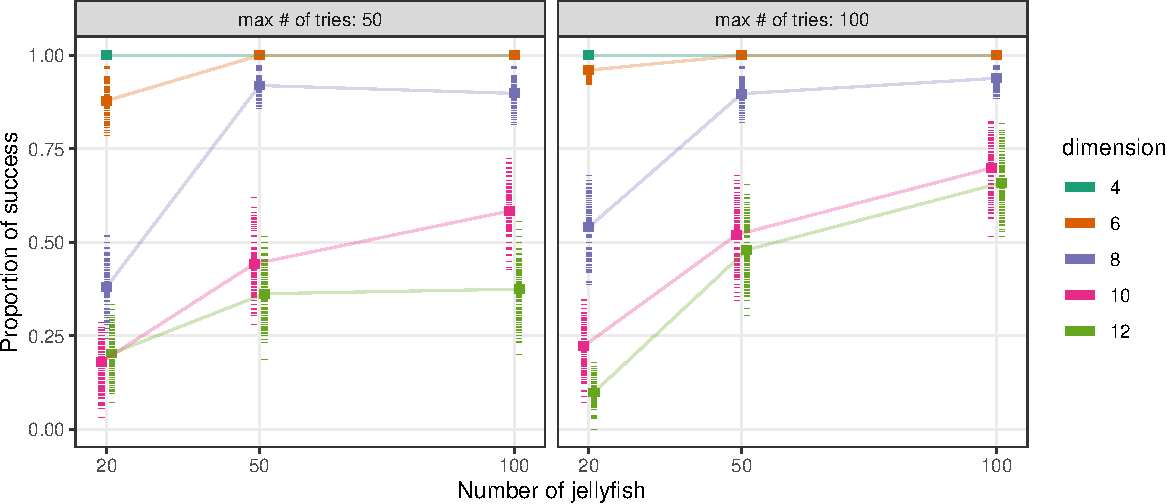
\includegraphics{jso_files/figure-pdf/fig-proportion-1.pdf}

}

\caption{\label{fig-proportion}Proportion of simulations reaches
near-optimal index values in the pipe-finding problem using the holes
index. The proportion is calculated based on the number of simulations,
out of 50, that achieve an index value within 0.05 of the
best-performing simulation. As the dimensionality increases, the
proportion of simulations reaching the optimal index value increases.}

\end{figure}%

The index properties, including smoothness and squintability, offer
numerical metrics to characterise the complexity of projection pursuit
optimisation problems. Table~\ref{tbl-smoothness-squintability} presents
the parameters for calculating both metrics estimated from the Gaussian
process (variance, range, smooth, and nugget) and the scaled logistic
function (\(\theta_1\) to \(\theta_4\)) for each case considered in the
simulation. The column ``smooth'' is used as the smoothness metric and
the column ``squint'' is calculated as equation
\ref{eq-squintability-parametric} as the squintability metric.
Table~\ref{tbl-mod-output} presents the results of fitting a generalised
linear model with a binomial family and a logit link function to a
sample of data in Table~\ref{tbl-mod-data}, where all the three
components (success rate, JS hyper-parameters, and index properties) are
combined. The model suggests that JSO success rate is positively
associated with the two hyper-parameters, as well as with the index
properties: smoothness and squintability. Specifically, using 10 more
jellyfish and 10 more tries increases the odd ratio of success by
24.11\% and 11.93\%, respectively. However, being flagged with long
runtime and an increase of data dimension reduce the success rate by
41.72\% and 53.36\%, respectively. The variable \texttt{squintability}
and \texttt{dimension} are significant, suggesting their importance
relative to JSO hyper-parameters in the optimisation success. In
defining a projection pursuit problem, factors such as the
shape-to-find, the index function used, and the data dimension,
determine the properties such as smoothness and squintability. These
metrics can then be compared across different problems to understand
their relative complexites. The results suggest that squintability has a
more significant influence than smoothness on the success rate of JSO.
Once the characteristics of the projection pursuit problem are fully
understood, increasing JSO hyper-parameters can enhance the search
effectiveness, however, it is also important to consider the resulting
increase in computational complexity.

\begin{table}

\caption{\label{tbl-smoothness-squintability}Parameters estimated from
the Gaussian process (including variance, range, smoothness, and nugget)
and scaled logistic function (\(\theta_1\) to \(\theta_4\)) for the
pipe-finding and sine-wave finding problems. The column ``smooth'' and
``squint'' represent the smoothness and squintability measures.}

\centering{

\centering\begingroup\fontsize{10}{12}\selectfont

\begin{tabular}{|>{}lll>{}r|rrr>{}r|rrrr>{}r|}
\toprule
  & shape & index & d & variance & range & smooth & nugget & $\theta_1$ & $\theta_2$ & $\theta_3$ & $\theta_4$ & squint\\
\midrule
1 & pipe & holes & 6 & 0.00 & 0.37 & 2.36 & 0.22 & 1.02 & 0.86 & 3.37 & 0.02 & 3.05\\
2 & pipe & holes & 8 & 0.00 & 0.18 & 2.19 & 0.82 & 1.01 & 0.87 & 3.26 & 0.03 & 2.96\\
3 & pipe & holes & 10 & 0.00 & 0.11 & 2.19 & 3.03 & 1.02 & 0.88 & 3.15 & 0.02 & 2.95\\
4 & pipe & holes & 12 & 0.00 & 0.15 & 2.29 & 1.58 & 1.01 & 0.88 & 3.34 & 0.00 & 3.12\\
5 & sine & MIC & 6 & 0.02 & 0.09 & 2.46 & 0.08 & 0.89 & 0.57 & 1.62 & -0.02 & 1.26\\
6 & sine & MIC & 8 & 0.02 & 0.08 & 2.64 & 0.08 & 0.93 & 0.33 & 1.31 & -0.03 & 0.77\\
7 & sine & TIC & 6 & 0.12 & 0.11 & 2.44 & 0.09 & 0.95 & 0.54 & 1.72 & -0.03 & 1.32\\
8 & sine & TIC & 8 & 0.12 & 0.10 & 2.47 & 0.09 & 0.95 & 0.56 & 1.72 & -0.03 & 1.37\\
9 & sine & dcor2d & 6 & 0.03 & 0.17 & 2.66 & 0.11 & 0.95 & 1.04 & 2.74 & -0.02 & 2.95\\
10 & sine & loess2d & 6 & 0.08 & 0.34 & 1.99 & 0.31 & 1.02 & 1.04 & 2.65 & 0.08 & 2.76\\
11 & sine & splines2d & 6 & 0.04 & 0.24 & 2.54 & 0.10 & 1.01 & 1.05 & 2.73 & -0.01 & 3.12\\
12 & sine & stringy & 6 & 0.00 & 0.01 & 1.54 & 38.17 & 1.05 & 0.01 & 254.73 & 0.05 & 2.96\\
\bottomrule
\end{tabular}
\endgroup{}

}

\end{table}%

\begin{table}

\caption{\label{tbl-mod-data}The first 7 rows of the datasets processed
for modelling.}

\centering{

\centering\begingroup\fontsize{10}{12}\selectfont

\begin{tabular}{lrrrrrrr}
\toprule
index & d & smoothness & squintability & n. jellyfish & max. tries & success rate & time (sec)\\
\midrule
MIC & 6 & 2.46 & 1.26 & 20 & 50 & 0.12 & 2.48\\
MIC & 6 & 2.46 & 1.26 & 20 & 100 & 0.24 & 8.95\\
MIC & 6 & 2.46 & 1.26 & 50 & 50 & 0.52 & 5.65\\
MIC & 6 & 2.46 & 1.26 & 50 & 100 & 0.64 & 13.22\\
MIC & 6 & 2.46 & 1.26 & 100 & 50 & 0.76 & 19.45\\
MIC & 8 & 2.64 & 0.77 & 20 & 50 & 0.08 & 2.57\\
MIC & 8 & 2.64 & 0.77 & 20 & 100 & 0.08 & 4.96\\
\bottomrule
\end{tabular}
\endgroup{}

}

\end{table}%

\begin{table}

\caption{\label{tbl-mod-output}Model estimates of proportion of
jellyfish success on index properties and jellyfish hyper-parameters
from the generalised linear model with a binomial family and a logit
link function. The variable smoothness, squintability, number of
jellyfish and maximum number of tries are positively associated with JSO
success rate while data dimension and being flagged as long runtime are
negatively associated with the success rate. The variable squintability
and dimension are significant, suggesting their importance relative to
jellyfish hyper-parameters in the optimisation success.}

\centering{

\centering\begingroup\fontsize{10}{12}\selectfont

\begin{tabular}{|>{}lrrr>{}r|}
\toprule
term & estimate & std.error & statistic & p.value\\
\midrule
Intercept & -4.52 & 5.33 & -0.85 & 0.40\\
Smoothness & 1.19 & 1.92 & 0.62 & 0.53\\
Squintability & 2.06 & 0.68 & 3.01 & 0.00\\
Dimension (d) & -0.63 & 0.26 & -2.46 & 0.01\\
Long time & -0.87 & 1.29 & -0.68 & 0.50\\
N. jellyfish & 0.22 & 0.13 & 1.70 & 0.09\\
Max. tries & 0.11 & 0.15 & 0.75 & 0.45\\
\bottomrule
\end{tabular}
\endgroup{}

}

\end{table}%

\section{Conclusion}\label{sec-conclusion}

This paper has presented new metrics to mathematically define desirable
features of PP indexes, squintability and smoothness, and used these to
assess the performance of the new jellyfish search optimiser. The
metrics will be generally useful for characterising PP indexes, and help
with developing new indexes.

In the comparison of the JSO against the currently used CRS, as expected
the JSO vastly out-performs CRS, and provides a high probability of
finding the global optima. The JSO obtains the maximum more cleanly,
with a slightly higher index value, and plot of the projected data
showing the structure more clearly.

The JSO performance is affected by the hyper-parameters, with a higher
chance of reaching the global optima when more jellyfish are used and
the maximum number of tries is increased. However, it comes at a
computational cost, as expected. The performance declines if the
projection dimension increases and if the PP index has low
squintability. The higher the squintability the better chance the JSO
can find the optima. However, interestingly smoothness does not affect
the JSO performance.

The new JSO is integrated with the current implementation of the
projection pursuit guided tour in the \texttt{tourr} package, and can be
further examined using PP optimisation diagnostics in the \texttt{ferrn}
package. Using the JSO is a little different than the current CRS,
because it runs many paths. The recommended approach is to conduct the
optimisation off-line, extract the bases of a selected jellyfish, and
then use the planned tour to follow selected jellyfish. The tools for
this are available in the \texttt{tourr} package, too.

\section{Acknowledgement}\label{acknowledgement}

The article is created using Quarto \citep{Allaire_Quarto_2022} in R
\citep{R}. The source code for reproducing the work reported in this
paper can be found at:
\url{https://github.com/huizezhang-sherry/paper-jso}. Nicolas Langrené
acknowledges the partial support of the Guangdong Provincial Key
Laboratory IRADS (2022B1212010006, R0400001-22) and the UIC Start-up
Research Fund UICR0700041-22.


\renewcommand\refname{References}
  \bibliography{bibliography.bib}


\end{document}
